\documentclass[11pt, letterpaper, titlepage]{article}
\usepackage[utf8]{inputenc}
\usepackage{geometry}
\usepackage{color,graphicx,overpic} 
\usepackage{fancyhdr}
\usepackage{amsmath,amsthm,amsfonts,amssymb}
\usepackage{mathtools}
\usepackage{hyperref}
\usepackage{multicol}
\usepackage{array}
\usepackage{float}
\usepackage{blindtext}
\usepackage{longtable}
\usepackage{scrextend}
\usepackage[font=small,labelfont=bf]{caption}
\usepackage[framemethod=tikz]{mdframed}
\usepackage{calc}
\usepackage{titlesec}
\usepackage{listings}
\usepackage[normalem]{ulem}
\usepackage{tabularx}
\usepackage{mathrsfs}
\usepackage{bookmark}
\usepackage{apple_emoji}
\usepackage{setspace}
\usepackage{enumitem}
\usepackage{adjustbox}
\usepackage{booktabs}

\graphicspath{ {images/} }
 
\allowdisplaybreaks

\definecolor{mycolor}{rgb}{0, 0, 0}

\geometry{top=2.54cm, left=2.54cm, right=2.54cm, bottom=2.54cm}
\setlength{\headheight}{20pt}
\setlength{\parskip}{0.6cm}
\setlength{\parindent}{1cm}

\title{\textbf{\Huge{
\begin{center}
    STAT 235\\ 
    Lab 1\\
\end{center}
}}}
\author{
    Name: \B enjamin Kong\\
    ID: 1573684\\
}

\newcommand{\B}{
\includegraphics[height=1.5em, valign=B, raise=-0.2em]{BigB.png}} 

\pagestyle{fancy}
\fancyhf{}
\rhead{\B enjamin Kong | 1573684}
\lhead{\textit{STAT 235 Lab 1}}
\rfoot{Page \thepage}

\begin{document} 
\doublespacing
\maketitle

\begin{enumerate}
    \item \begin{enumerate}[parsep=0.4cm]
        \item The type of golf ball affects how far it travels (each ball type may be a different size, different weight, have different aerodynamic properties, be more compressible, etc.). 
        
        The two types of balls were launched alternately in order to reduce discrepancy in the data. For example, if we launch all the balls of the first type and then launch the balls of the second type after, the wind may vary between the long period during which we are only launching the first type of ball. By alternating the balls, the discrepancy is reduced, giving more reliable data.

        \item We could use the results of the study for a scenario where the conditions are similar to the test. However, the results can't be extended to all conditions. If the conditions in this test were windy and the first ball performed better under windy conditions because it was heavier, this doesn't mean it would outperform the second ball if it wasn't windy and the second ball was lighter.
    \end{enumerate}

    \item \begin{enumerate}
        \item The plot for the line chart of carry is displayed in figure \ref{2a}. Overall, the plot is trending up (confirmed through creating a trendline in Excel).
        
        \begin{figure}
            \centering
            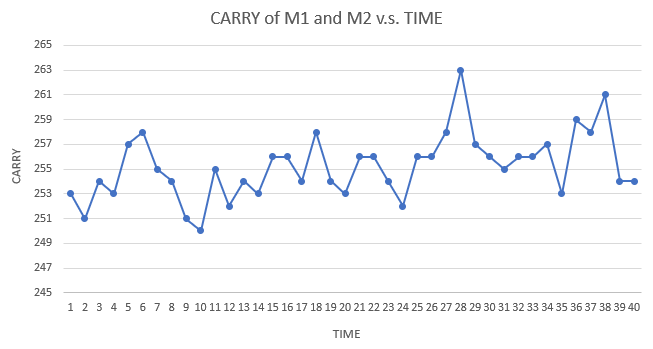
\includegraphics[width=0.9\textwidth]{2a.PNG}
            \caption{Carry of the two balls (M1 and M2) as a function of time.}
            \label{2a}
        \end{figure}

        \item The plot for the two line charts for the carries for each type of ball are displayed in figure \ref{2b}. From eyeballing the plot, it looks like the center for M1 is about 255 and the variability looks low compared to M2. It looks like the center for M2 is about 257 and the variability looks significant compared to M1.
        
        \begin{figure}
            \centering
            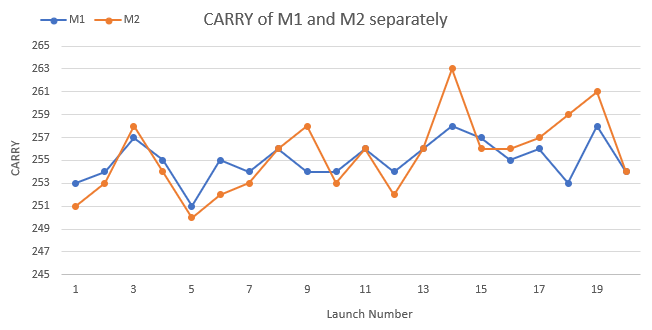
\includegraphics[width=0.9\textwidth]{2b.PNG}
            \caption{Carry of each ball type. The blue line is the first ball (M1) and the orange line is the second ball (M2).}
            \label{2b}
        \end{figure}
    \end{enumerate}

    \item \begin{enumerate}
        \item The histogram for the carry of M1 is displayed in figure \ref{3a}.
        
        \begin{figure}
            \centering
            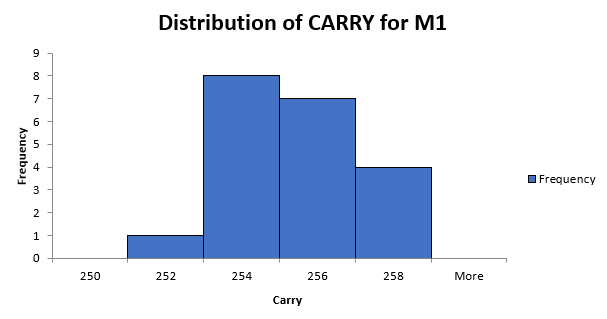
\includegraphics[width=0.6\textwidth]{3a.PNG}
            \caption{Distribution of carry for ball type M1.}
            \label{3a}
        \end{figure}

        \item The histogram for the carry of M1 is displayed in figure \ref{3b}. 
        
        \begin{figure}
            \centering
            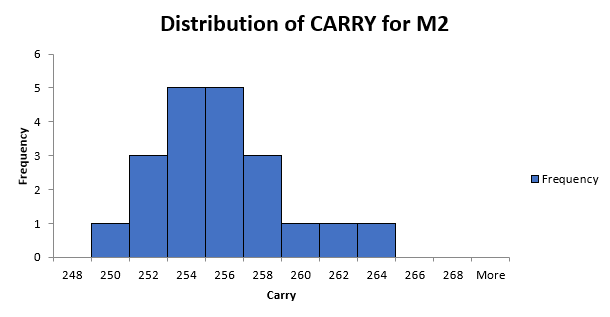
\includegraphics[width=0.6\textwidth]{3b.PNG}
            \caption{Distribution of carry for ball type M2.}
            \label{3b}
        \end{figure}

        \item The shapes of both histograms are right skewed (the tail of the distribution is on the right side). The conclusions are consistent with the plot in part (b) of question 2. For example, the larger variance of M2 seen in figure \ref{2b} is evident from larger spread of the histogram for M2. There are no outliers in the plots.
    \end{enumerate} 

    \item \begin{enumerate}
        \item The results from Descriptive Statistics from Excel are displayed in table \ref{4a}.
        
        \begin{table}[]
            \centering
            \caption{The Descriptive Statistics for M1 and M2 retrieved from Excel.}
            \begin{tabular}{@{}lll@{}} \toprule
                & M1       & M2       \\ \midrule
                Mean               & 255      & 255.4    \\
                Standard Error     & 0.39736  & 0.748331 \\
                Median             & 255      & 256      \\
                Mode               & 254      & 256      \\
                Standard Deviation & 1.777047 & 3.34664  \\
                Sample Variance    & 3.157895 & 11.2     \\
                Kurtosis           & 0.024837 & 0.023128 \\
                Skewness           & -0.12505 & 0.520104 \\
                Range              & 7        & 13       \\
                Minimum            & 251      & 250      \\
                Maximum            & 258      & 263      \\
                Sum                & 5100     & 5108     \\
                Count              & 20       & 20       \\ \bottomrule
            \end{tabular}
            \label{4a}
        \end{table}
    \end{enumerate}
\end{enumerate}

\end{document}
